
%%% Local Variables: 
%%% mode: latex
%%% TeX-master: "report_dMRI_preprocessing.tex"
%%% End: 

\section{Reconstruction}
\label{sec:reconstruction}
From the actual dMRI data we can create the \emph{tractrography}, the \emph{fractional anisotropy} (FA) volume and the \emph{mean diffusivity} (MD) volume.
A tractography is created in two steps: reconstruction and tracking. Reconstruction is about computing the information about the spatial distribution of the diffusion signal within each voxel. While tracking tries to connect many signals to form a tractography based on orientation signal of each voxel. In this paragraph, the main focus is on how to reconstruction of dMRI data.   

However, before doing reconstruction, the actual dMRI data in NIfTI image needs to extract brain image only. Because the result of scanner usually contains not only brain but also other things close to brain which can distract the processing of tracking. Brain extraction is the process of removing the skull and the rest of the head from the brain, therefore is necessary to be done before further analysis. Example of brain extraction can be seen in figure \ref{Fig:bet}. The resulting file only contains a representation of the brain's anatomy.

\begin{figure} 
  \centering 
  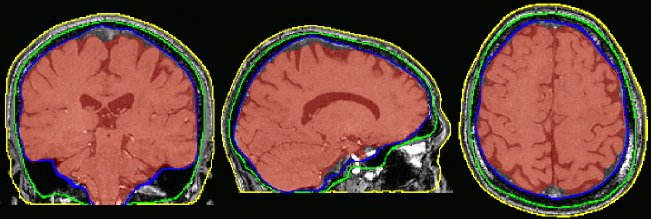
\includegraphics[width=10cm]{bet.jpg}
  \caption{Brain extraction}
  \label{Fig:bet}
\end{figure}

Brain extraction can be done with the FSL program BET (Brain Extraction Tool)~\cite{smith2002automated}. FSL\footnote{\url{http://www.fmrib.ox.ac.uk/fsl/index.html}} is a comprehensive library of analysis tools for FMRI, MRI and DTI brain imaging data. FSL is written mainly by members of the Analysis Group, FMRIB, Oxford, UK. FSL runs on Apple and PCs (Linux and Windows), and is very easy to install. Most of the tools can be run both from the command line and as GUIs ("point-and-click" graphical user interfaces).

BET~\cite{smith2002automated} takes an image of a head and removes all non-brain parts of the image. It uses a deformable model that evolves to fit the brain's surface by the application of a set of locally adaptive model forces. This method is very fast and requires no preregistration or other pre-processing before being applied. Result of this is a file saved with a ‘brain’ extension at its end. BET can run from the console (with the command bet). FSL recommend that do not use the BET-GUI because it almost always needs options that are not available in the GUI. Also always use FSLView to inspect the output of the bet procedure and to fine-tune the bet operation. Run bet in the console to see the available options and its command line:

\begin{python}
 bet(<ori_NIfTI_image_file>, <brain_extract_file>)
\end{python}

The result of BET can be seen in the bottom line of the figure ~\ref{Fig:subj3}. This image is taken from subject 3 of the Cambridge dataset. While origional image date is in the top line of this figure ~\ref{Fig:subj3}.

\begin{figure} 
  \centering 
  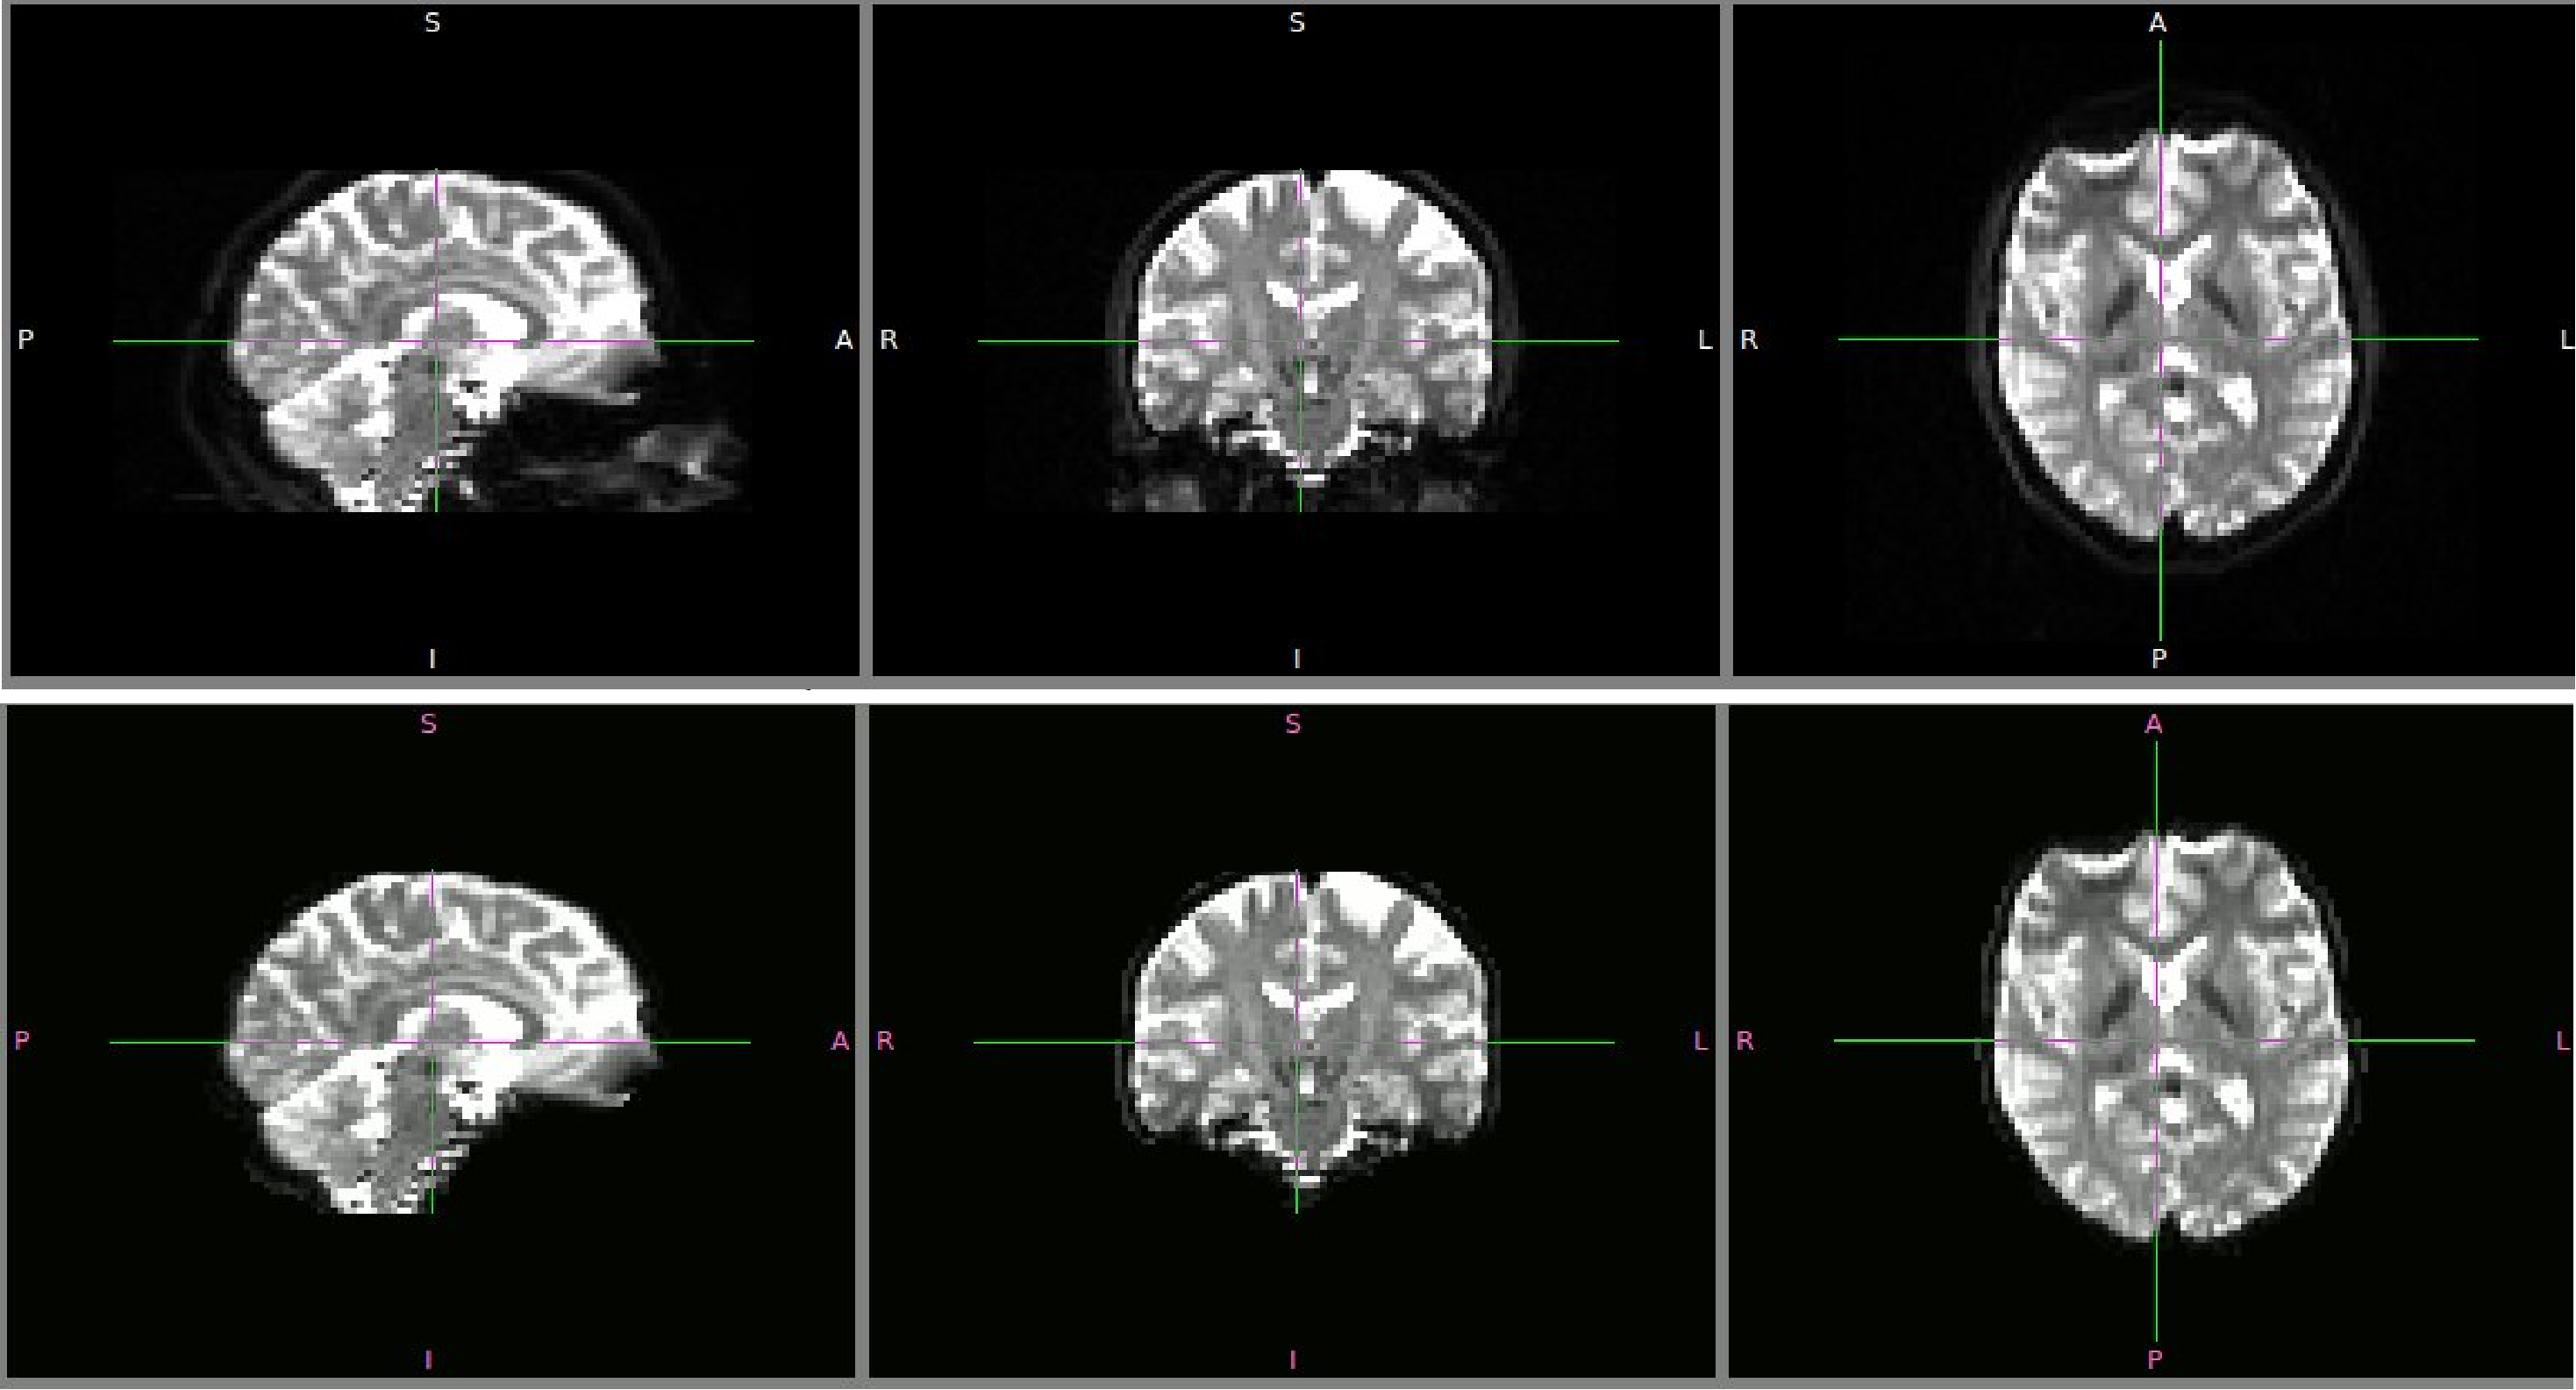
\includegraphics[width=13.5cm]{subj3cambridge.pdf}   %#{rawsubj3.jpg}
  \caption{Origional NIfTI (top) and BET (bottom) image file of subject 3 in Cambridge datase}
  \label{Fig:subj3}
\end{figure}

%\begin{figure} 
%  \centering 
%  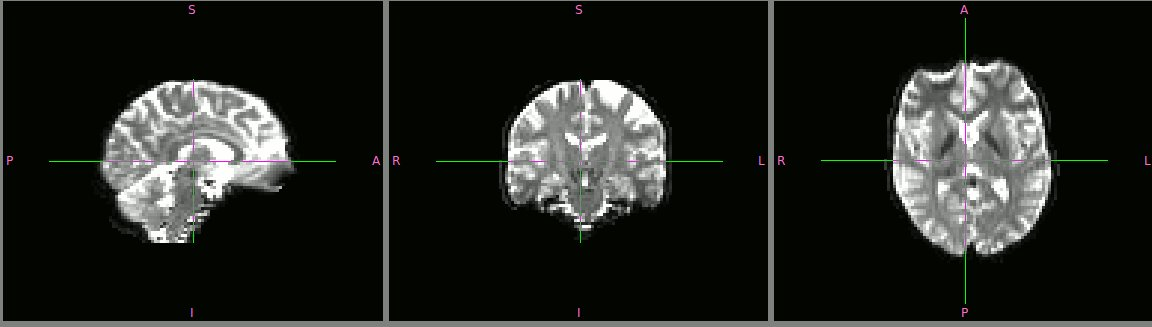
\includegraphics[width=13cm]{betsubj3.jpg}
%  \caption{After brain extraction by BET of subject 3 in Cambridge datase}
%  \label{Fig:betsubj3}
%\end{figure}

After brain extraction, we can do reconstruction step. The main purpose of this is to estimate the orientation information from the diffusion signal within each voxel which is adequate for accurate tractography generation. In the last few years, an increasing number of techniques have been proposed to recover the signal directions inside the voxel from diffusion MRI data. The most simple methods is Diffusion Tensor model proposed by Basser et. al
~\cite{basser1994diffusion}. But in many cases this model is not sufficiently, because most of voxels inside brain contain multiple fiber bundles crossings while this model is only working with single tensor. Many other reconstruction methods have been proposed to overcome the limitations of this Diffusion Tensor model. The earliest studies distinguished between voxels with isotropic, single-fiber anisotropic, and multi-fiber anisotropic complexity and have reported clustered and symmetric regions of increased complexity, supporting genuine effects consistent with anatomical knowledge. Following are some other advanced methods such as Diffusion Spectrum Imaging ~\cite{callaghan1988microscopy} or Higher Order Tensors~\cite{ozarslan2005diffusion}. The overview of these model can be found more detail in~\cite{hagmann2006diffusion} or \footnote{\url{http://radiographics.rsna.org/content/26/suppl_1/S205.full}}. The basic idea for diffusion tensor model is briefly described in the following.

\begin{figure} 
  \centering 
  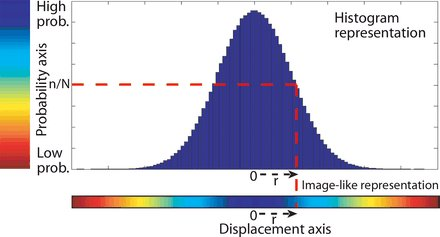
\includegraphics[width=12cm]{diffusion1.jpg}
  \caption{Histogram of displacement distribution}
  \label{Fig:diffusion1}
\end{figure}

The histogram in figure~\ref{Fig:diffusion1} shows a typical displacement distribution in a one-dimensional model. All the molecules have moved the given distance r. For each displacement distance r (x-axis) there is a corresponding probability n/N (y-axis), which is the proportion of molecules within a voxel that were displaced that distance within a time interval $\Delta$ (the duration of the diffusion experiment). The top of the histogram is centered on zero, indicating that most molecules had the same position at $t = 0$ and $t = \Delta$. The proportion of molecules that traveled the given distance r is indicated by the dotted red line. The horizontal color bar, in which blue signifies a high probability and red a low probability of displacement, shows the same Gaussian distribution. 

\begin{figure} 
  \centering 
  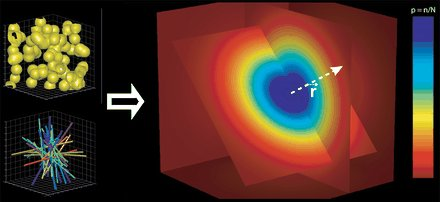
\includegraphics[width=8cm]{diffusionprobability.jpg}
  \caption{The 3D diffusion probability density function in a voxel which contains intersect orientations}
  \label{Fig:diffusion_intersect}
\end{figure}


But, a histogram like in figure~\ref{Fig:diffusion_intersect} is adequate for the display of one-dimensional data, because it is not practical for visualizing displacement in multiple dimensions. A useful approach is instead to color-code the probability. With such a representation, the one-dimensional problem can be visualized as a colored displacement axis (x-axis) in which blue codes for high and red for low probability (figure~\ref{Fig:diffusion1}). According to this rule, we can represent actual three-dimensional (3D) diffusion as a 3D image in which the probability of displacement in three intersecting planes is coded in color (figure~\ref{Fig:diffusion_intersect}). The central voxel of the image is the origin, and its value codes for the probability, or the proportion of molecules (n/N) that do not undergo displacement between $t = 0$ and $t = \Delta$. This 3D diagram represents the displacement distribution. On a photograph taken at $t = \Delta$, the dye will have been diluted (diffused), and the relative color density will indicate the proportion of dye molecules displaced a given distance.

Diagram shows the 3D diffusion probability density function in a voxel that contains spherical cells (top left) or randomly oriented tubular structures that intersect, such as axons (bottom left). This 3D displacement distribution, which is roughly bell shaped, results in a symmetric image (center), as there is no preferential direction of diffusion. The distribution is similar to that in unrestricted diffusion but narrower because there are barriers that hinder molecular displacement. The center of the image (origin of the r vector) codes for the proportion of molecules that were not displaced during the diffusion time interval. The color bar (right) shows the spectrum used in color coding to represent probability, from the lowest value, which is indicated by red, to the highest, which is indicated by blue. 

\begin{figure} 
  \centering 
  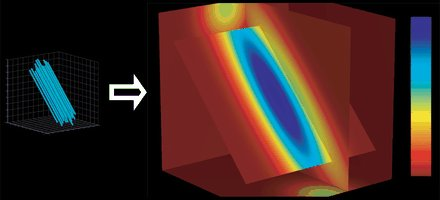
\includegraphics[width=8cm]{diffusionalign.jpg}
  \caption{The 3D diffusion probability density function in a voxel in which orientation alignes with the axons}
  \label{Fig:diffusion_allign}
\end{figure}

The figure~\ref{Fig:diffusion_allign} shows the diffusion probability density function within a voxel in which all the axons are aligned in the same direction. The displacement distribution is cigar shaped and aligned with the axons. 

\begin{figure} 
  \centering 
  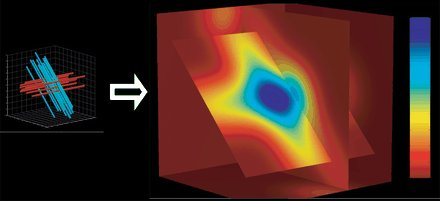
\includegraphics[width=8cm]{diffusionorthogonal.jpg}
  \caption{The 3D diffusion probability density function in a voxel with fibers intersecting at an angle of 90°}
  \label{Fig:diffusion_orthogonal}
\end{figure}

While the diagram in figure~\ref{Fig:diffusion_orthogonal} shows the diffusion probability density function within a voxel that contains two populations of fibers intersecting at an angle of 90°. The molecular displacement distribution produces a cross shape. Diffusion in a homogeneous medium is well described as having a Gaussian distribution. Depending on the type of molecule, the temperature of the medium, and the time allowed for diffusion, the distribution will be wider or narrower. The spread of the Gaussian distribution is controlled by a single parameter: variance $(\sigma
^{2})$. Variance, in turn, depends on two variables, so that $\sigma^{2} = 2\cdot D\cdot \Delta $, where $\Delta$, the diffusion coefficient, characterizes the viscosity of the medium or the ease with which molecules are displaced. The longer the diffusion time interval, the larger the variance, because there is more time in which molecules may be displaced.

\begin{figure} 
  \centering 
  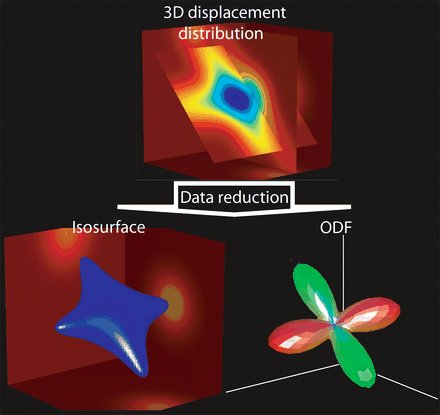
\includegraphics[width=5cm]{orientationdistributionfunction.jpg}
  \caption{Two approaches for visual representation of 3D diffusion data}
  \label{Fig:orientation_distribution_function}
\end{figure}
Typically, at diffusion imaging, there is less interest in obtaining a detailed diffusion profile than in determining the direction of the most rapid diffusion, because the latter parameter likely corresponds to the orientation of axons or other fibrillar structures. One possible approach would be to replace the diffusion probability density function with an isosurface, which is a surface that passes through all points of equal value, or, in other words, where the value of ƒ(r) is a constant (figure~\ref{Fig:orientation_distribution_function}). A more commonly used technique that is less sensitive to noise involves the computation of the orientation distribution function from the displacement distribution.

\begin{figure} 
  \centering 
  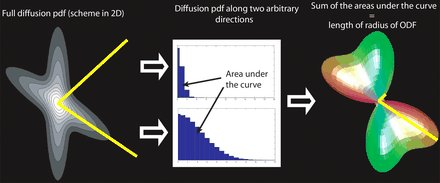
\includegraphics[width=11cm]{computeODF.jpg}
  \caption{How to compute ODF}
  \label{Fig:compute_ODF}
\end{figure}

Figure~\ref{Fig:orientation_distribution_function} shows two approaches that may be used to simplify the visual representation of 3D diffusion data: replacement of the displacement distribution with an isosurface, and computation of the orientation distribution function (ODF). And figure~\ref{Fig:compute_ODF} shows how an orientation distribution function (ODF) is computed and represented. The left image is a section through a schematized 3D displacement distribution. The value of the orientation distribution function is computed along two axes (yellow lines). While the center one is histogram that represents the displacement distribution along the two axes. The value of the orientation distribution function along those axes equals the area under the curve for each axis. In this example, the two areas under the curve are respectively small and large, indicating that there is much less diffusion in the one direction than in the other. In the right image, the sum of the areas under the curve is represented by a deformed sphere in which the lengths of the two radii (yellow lines) are short and long, corresponding to little diffusion and much diffusion, respectively. To compute the orientation distribution function, the area under the curve is computed for every direction.

\begin{figure} 
  \centering 
  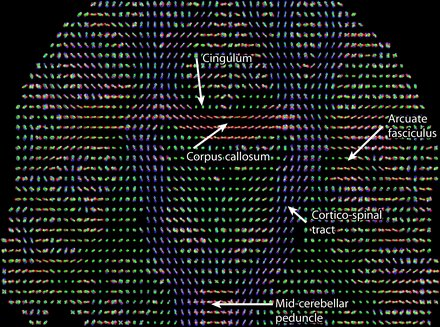
\includegraphics[width=8cm]{ODFmap.jpg}
  \caption{Orientation distribution function map of a coronal brain section}
  \label{Fig:ODF_map}
\end{figure}

An orientation distribution function may be considered a deformed sphere whose radius in a given direction is proportional to the sum of values of the diffusion probability density function in that direction. For ease of visualization, we color code the surface according to the diffusion direction ([x,y,z] = [r,b,g], where r = red, b = blue, and g = green). An orientation distribution function or isosurface can be plotted for each individual MR imaging voxel in a section. In the figure~\ref{Fig:ODF_map}, for every brain position p, an orientation distribution function is plotted to characterize the local diffusion probability density function. It is easy to identify the corticospinal tract, in which the dominant color is blue, and the corpus callosum, in which red is predominant. More difficult to see are the cingulum and the arcuate fasciculus, depicted predominantly in green, and the middle cerebellar peduncle, in red. From this, we can easy to tracking tractography. But more detail will be discuss on the next paragraph about tracking.

MR imaging is the result of the application of gradients in different directions and with different intensities at specific moments of the acquisition sequence. The values of the measured signal are organized in a coordinate system known as k-space. Performing the acquisition enables the filling of k-space. To transform the raw MR imaging data from k-space into a position-encoded visual image, a mathematical operation known as a Fourier transform is applied. Figure~\ref{Fig:MRI_obtain} shows the process with which a standard position-encoded MR image is obtained. First, the MR signal that was generated by the application of phase and frequency encoding gradients is sampled to fill k-space (a coordinate system used to organize the signal measurements). Next, the raw data (k-space images) are subjected to a mathematical operation known as a Fourier transform to reconstruct an image in the standard position space.
\begin{figure} 
  \centering 
  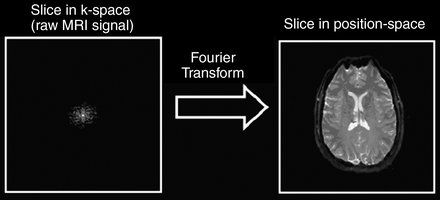
\includegraphics[width=8cm]{MRIobtain.jpg}
  \caption{The process to obtain a standard position-encoded MR image}
  \label{Fig:MRI_obtain}
\end{figure}

The application of a single pulsed gradient spin-echo (SE) sequence produces one diffusion-weighted image. This diffusion gradient can be represented as a 3D vector q whose orientation is in the direction of diffusion and whose length is proportional to the gradient strength. And the coordinates which are defined by all these vector q are called \textbf{q-space}. The gradient strength, or more often the diffusion weighting, is sometimes expressed in terms of the \textbf{b value}, which is proportional to the product of the square of the gradient strength q and the diffusion time interval $(b\approx q^{2}\Delta)$. One diffusion-weighted image corresponds to one position in q-space or, more precisely, that depicts the diffusion-weighted signal intensity in a specific position q for every brain position. Repeated applications of the sequence with gradients that vary in strength and in direction (ie, with variations of q) allow data sampling throughout q-space. Like the data from conventional MR imaging, in which a Fourier transform is applied to the data in k-space, the q-space data are subjected to a Fourier transform in every brain position. The result is a displacement distribution in each brain position (ie, voxel). In other words, a single application of the pulsed gradient SE sequence produces one brain image with a given diffusion weighting. Multiple repetitions of the sequence, each with a different diffusion weighting, are necessary to sample the entirety of q-space; the result is hundreds of brain images, each of which reflects the particular diffusion weighting used. One must then imagine that the data are reorganized so that in every brain position there is a q-space signal sample that consists of hundreds of values and that in every brain position a Fourier transform relates the raw q-space data to the diffusion probability density function 

\begin{figure} 
  \centering 
  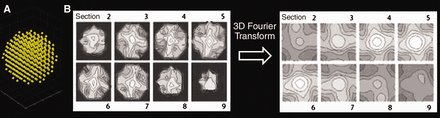
\includegraphics[width=13cm]{PDFprobabilitydensityfunction.jpg}
  \caption{The process to obtain a standard position-encoded MR image}
  \label{Fig:pdf}
\end{figure}

The diagram in figure~\ref{Fig:pdf} shows the process with which a 3D diffusion probability density function is obtained for one voxel (one brain position). In A, a 3D grid that represents q-space, each yellow dot corresponds to an MR signal sampling point. The signal is sampled at each point by varying the direction and strength of the diffusion gradient (q vector) of the pulsed gradient SE sequence. With a single application of the pulsed gradient SE sequence, one point in q-space is sampled for each brain position simultaneously, and the result is one diffusion-weighted image. In B, the left panel shows sections through the MR signal sampled in q-space for a specific brain position (one voxel), and the right panel shows the diffusion probability density function in the same voxel after a 3D Fourier transform of the MR signal in q-space is performed. The cross-shaped appearance of the diffusion probability density function is often seen in voxels in the brainstem, where axons of the corticospinal tract cross with axons of the middle cerebellar peduncle.

\begin{figure} 
  \centering 
  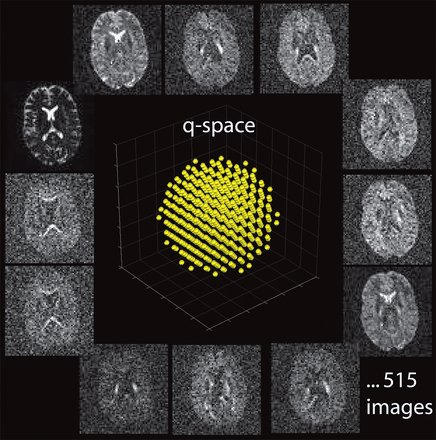
\includegraphics[width=5cm]{qspace.jpg}
  \caption{Q-space example}
  \label{Fig:qspace}
\end{figure}

Series of diffusion-weighted MR brain images are obtained with variations in the direction and strength of the diffusion gradient in the pulsed gradient SE sequence (figure ~\ref{Fig:qspace}). Each image shows the signal sampled at one point in q-space (one yellow dot). Every sampling point in q-space corresponds to a specific direction and strength of the diffusion gradient.

To describe the parameters applied in sampling q-space, the term “b value” is often used. The b value is proportional to the product of the diffusion time interval and the square of the strength of the diffusion gradient. All diffusion images should be compared with a reference image that is not diffusion weighted (a standard SE image)—in other words, one for which the strength of the diffusion gradient is zero (q = 0 and b = 0).

\begin{figure} 
  \centering 
  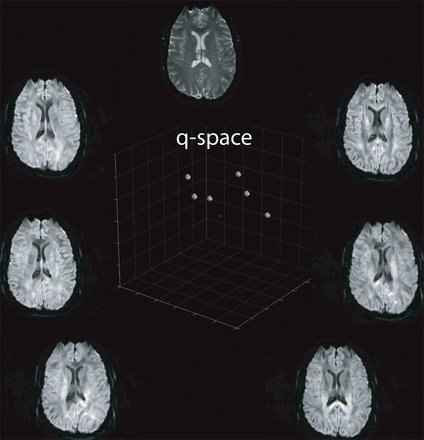
\includegraphics[width=6cm]{tensorqspace.jpg}
  \caption{Series of diffusion-weighted images obtained for diffusion tensor imaging}
  \label{Fig:tensor_qspace}
\end{figure}

When we sample at least six points in q-space with $q\neq0$  (diffusion-weighted images) and one point with q = 0 (reference image), we solve a set of six equations and the result is a diffusion tensor that is proportional to the Gaussian covariance matrix ~\cite{bihan2001tensor}. This diffusion tensor is a $3 \times 3$ matrix that fully characterizes diffusion in 3D space, assuming that the displacement distribution is Gaussian. The diffusion tensor is usually represented by an ellipsoid or an orientation distribution function. Figure~\ref{Fig:tensor_qspace} describes a series of diffusion-weighted images obtained for diffusion tensor imaging, in which q-space is sampled in at least six different directions and in which a non–diffusion-weighted reference image is obtained. The direction but not the strength of the diffusion gradient is changed for each sampling. 

\begin{figure} 
  \centering 
  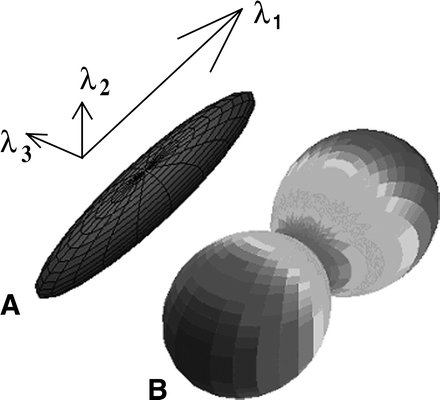
\includegraphics[width=5cm]{diffusiontensor.jpg}
  \caption{Two ways to present diffusion tensor}
  \label{Fig:diffusion_tensor}
\end{figure}


There are two ways to describe diffusion tensor. In figure~\ref{Fig:diffusion_tensor}, the diffusion tensor is shown as an ellipsoid (an isosurface) with its principal axes along the eigenvectors $(\lambda_{1}, \lambda_{2}, \lambda_{3})$. While in B, the diffusion tensor is shown as an orientation distribution function. 

The direction of the diffusion maximum is called the principal direction of diffusion and can be directly obtained by computing eigenvectors and eigenvalues of the tensor. Eigenvectors are orthogonal to one another, and, with eigenvalues, describe the properties of the tensor. Eigenvalues are ordered as $\lambda_{1}\geq \lambda_{2}\geq \lambda_{3}$, and each corresponds to one eigenvector. The eigenvector that corresponds to the largest eigenvalue $(\lambda_{1})$ is the principal direction of diffusion. If the eigenvalues are significantly different from each other, diffusion is said to be anisotropic (figure~\ref{Fig:diffusion_tensor}). If $\lambda_{1}$ is much larger than the second eigenvalue, $\lambda_{2}$, the diffusion is cigar shaped (figure~\ref{Fig:diffusion_tensor}). If $\lambda_{1}$ and $\lambda_{2}$ are similar but are much larger than $\lambda_{3}$, the diffusion is said to be planar or disc shaped. When all the eigenvalues are approximately equivalent, diffusion is isotropic and may be represented as a sphere ~\cite{westin2002processing}.

\begin{figure} 
  \centering 
  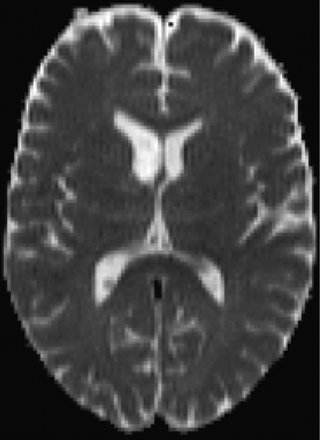
\includegraphics[width=5cm]{meandiffusion.jpg}
  \caption{Mean diffusion tensor image}
  \label{Fig:mean_diffusion}
\end{figure}

The mathematical properties of the diffusion tensor make it possible to extract several useful scalar measures from diffusion tensor images. The mean diffusion, also known as the trace, is computed by averaging the diagonal elements of the matrix~\cite{bihan2001tensor}(Equation:~\ref{Equ:MD}). The result is an image like that in figure~\ref{Fig:mean_diffusion}. Frequently, mean diffusivity (MD) is used instead of the trace defined as

\begin{equation}
   MD=\frac{trace(D)}{3}=\frac{\lambda_{1}+\lambda_{2}+\lambda_{3}}{3}
   \label{Equ:MD}	
\end{equation}

\begin{figure} 
  \centering 
  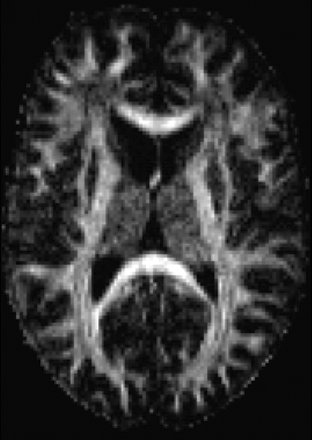
\includegraphics[width=5cm]{fractionalanisotrophy.jpg}
  \caption{The fractional anisotrophy image}
  \label{Fig:fractional_anisotrophy}
\end{figure}

The relationship between the eigenvalues reflects the characteristics of diffusion. To describe the shape of diffusion with a scalar value, fractional anisotropy is most often used~\cite{bihan2001tensor}. However, other measures, such as those described by Westin et al~\cite{westin2002processing}, are available. Fractional anisotropy is computed by comparing each eigenvalue with the mean of all the eigenvalues $(\langle \lambda \rangle)$, as in the following equation:
\begin{equation}
   FA=\frac{1}{\sqrt{2}}\frac{\sqrt{(\lambda_{1}-\lambda_{2})^{2}+(\lambda_{2}-\lambda_{3})^{2}+(\lambda_{3}-\lambda_{1})^{2}}}{\sqrt{\lambda_{1}^{2}+\lambda_{2}^{2}+\lambda_{3}^{2}}}
   \label{Equ:FA}	
\end{equation}
where FA is the fractional anisotropy. The fractional anisotropy of a section of diffusion tensors can be seen in figure~\ref{Fig:fractional_anisotrophy}. This image shows the fractional anisotropy, which is computed from the eigenvalues of the diffusion tensor. If FA is equal to 1 that means very anisotropic (infinitely prolonged ellipsoid or a ‘stick’) and if FA is equal to 0 that means completely isotropic (sphere). Whenever we are using FA volumes we are implicitly assuming that the propagator of the spin displacements in every voxel has a 3D Gaussian distribution. This assumption is used in most of the diffusion related literature where Diffusion Tensor Imaging is the prevailing term. Unfortunately, in reality things are much more complicated; inside our brain the axons are semi-permeable (restriction), the water molecules interact with many different elements in the complex intra fibre fluid, the fibres might cross, kiss, divert or bend inside a voxel or between voxels. Therefore, assuming a Gaussian distribution is a nontrivial approximation. However, FA is still prevalent as it is easy to calculate and it gives similar values across different acquisitions.

\begin{figure} 
  \centering 
  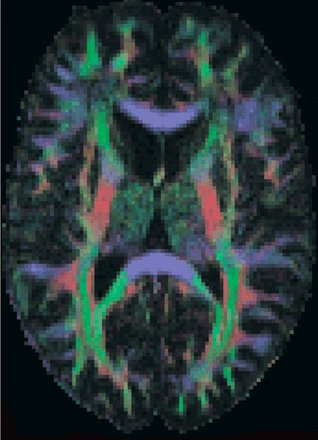
\includegraphics[width=5cm]{principaldirection.jpg}
  \caption{The principal direction of diffusion}
  \label{Fig:principal_direction_diffusion}
\end{figure}


The ellipsoid or the orientation distribution function is the most accurate method for visualizing the diffusion tensor data, but sometimes it is difficult to represent it over an imaging section on a display monitor~\cite{basser1994diffusion}. Color coding of the diffusion data according to the principal direction of diffusion may be a more practical way of visualizing the data~\cite{bihan2001tensor}. In the color coding system, red corresponds to diffusion along the inferior-superior axis (x-axis); blue, to diffusion along the transverse axis (y-axis); and green, to diffusion along the anterior-posterior axis (z-axis). The intensity of the color is proportional to the fractional anisotropy. An example of this color coding scheme is shown in figure~\ref{Fig:principal_direction_diffusion}. In this image, the color-coded part shows the orientation of the principal direction of diffusion, with red, blue, and green representing diffusion along x-, y-, and z-axes, respectively. The color intensity is proportional to the fractional anisotropy.

In general, diffusion tensor imaging (\textbf{DTI}) and q-ball imaging (\textbf{QBall}) are hypothesis-based simplifications that are used to shorten image acquisition time and reduce hardware requirements. They can be used to obtain maps of the orientation distribution functions. Care must be taken when interpreting diffusion tensor imaging data and q-ball imaging data, as there may be brain areas in which the underlying hypotheses are not applicable. In this experiment, we used DTI method to find orientation information of signal within each voxel. The implement of DTI has already been done in Dipy (Diffusion Imaging in Python)\footnote{\url{http://nipy.sourceforge.net/dipy/index.html}}. Actually, in Dipy, authors develop DTI algorithm basing on the work of Yeh. et. al ~\cite{yeh2010qsampling} who extends the current derivations for diffusion signal reconstruction and provides both scalar and vector metrics that facilitate the understanding of the underlying signal and its use for fast and accurate tractography. The key issue is the reentrance of the spin density as an important part of the diffusion voxel reconstruction. The spin density together with the diffusion propagator give rise to the spin propagator. From the spin propagator both old metrics like FA (equation~\ref{Equ:FA}) and MD (equation~\ref{Equ:MD}) can be calculated non-parametricly. Following will describe some basic command lines in Dipy for calculating tensor directionality.

\begin{itemize}
	\item \textbf{First, import the necessary modules}

\begin{description}
	\item[]
numpy is for numerical computation
\begin{python}
import numpy as np
\end{python}

	\item[]
nibabel is for data formats

\begin{python}
import nibabel as nib
\end{python}

	\item[]
dipy.reconst is for the reconstruction algorithms which we use to create directionality models for a voxel from the raw data

\begin{python}
import dipy.reconst.dti as dti
\end{python}

\end{description}

\item \textbf{Accessing the necessary datasets}(more detail can be found in section~\ref{sec:raw_to_nifti})
	
	\begin{description}
		\item[]
		Load the nifti file found at path fimg as an NIfTI image format 
		
\begin{python}
img = nib.load(nii_filename)
\end{python}

		\item[]
		Read the datasets from the NIfTI image format
\begin{python}
data = img.get_data()
\end{python}
		
		The raw diffusion weighted MR data is 4-dimensional, the last one is number of gradient directions while the first triple is the dimension of 3d volume.

		\item[]
		Read the affine matrix
\begin{python}
affine = img.get_affine()
\end{python}
		
		this gives the mapping between volume indices (voxel coordinates) and world coordinates.

		\item[]
		Read the b-values
\begin{python}
bvals=np.loadtxt(fbvals)
\end{python}

		this gives a function of the strength, duration, temporal spacing and timing parameters of the 	specific paradigm used in the scanner, one per gradient direction.

		\item[]
		Read the b-vectors
\begin{python}
gradients=np.loadtxt(fbvecs).T
\end{python}
		this is the unitary direction of the gradient.
		\item[]
		Note that \textit{fbvals} and \textit{fbvecs} are results from converting DICOM to NIfTI format.
	\end{description}
	
\item \textbf{Calculating models and parameters of directionality}

We are now set up with all the data and parameters to start calculating directional models for voxels and their associated parameters-FA (fractional anisotropy).

	\begin{description}
		\item[]
		Calculate the Single Tensor Model (STM)
\begin{python}
tensor=dti.Tensor(data,bvals,gradients,thresh=50) 
\end{python}

		\item[]
		Calculate Fractional Anisotropy (FA) from STM
\begin{python}
FA = tensors.fa()
\end{python}

		FA is a 3-d array with one value per voxel. Dimension of FA is equal to the dimension of the data volume.

	\end{description}
\end{itemize}

In this section, an overview of DTI - diffusion tensor image - one of the most popular and simple reconstruction method is presented. After that, we went to Dipy (diffusion imaging in python) command lines to create tensors and fractional anisotrophy which are necessary for tractography. The next part will discuss about theory of tracking methods and how to do it in python with help from Dipy.





